\documentclass[12pt]{article}

\usepackage[a4paper,margin=1in]{geometry}
\usepackage{setspace}
\onehalfspacing

\usepackage{amsmath,amssymb,amsthm}
\usepackage{graphicx}
\usepackage{float}
\usepackage{caption}
\usepackage{subcaption}
\usepackage{enumitem}

% \begin{figure}[H]
%     \centering
%     
\includegraphics[width=0.6\textwidth]{hw1_q2b_surface.png}
%     \caption{Optimal joint density f(p, d)}
%     \label{fig:2b}
% \end{figure}

\title{ECON 5345 Homework 8 Report}
\author{Harlly Zhou}
\date{\today}

\begin{document}

\maketitle

\noindent\textbf{Setup}: The central planner maximizes the following objective.
\begin{align*}
    \max_{C_t, K_t, L_t, I_t} \mathbb{E} \sum_{t=0}^{+\infty} \beta^t \bigg\{\frac{C_t^{1-\sigma}}{1-\sigma} - \frac{\xi L_t^{1+1/\eta}}{1+1/\eta}\bigg\},
\end{align*}
subject to
\begin{align*}
    Y_t &= Z_t K_{t-1}^{\alpha} L_t^{1-\alpha},\\
    Y_t &= C_t + I_t + \frac{\phi}{2} \left( \frac{K_t}{K_{t-1}} - 1 \right)^2 K_{t-1},\\
    K_t &= (1-\delta)K_{t-1} + I_t,\\
    Z_t &= e^{\varepsilon_t}Z_{t-1}^{\rho}, \varepsilon_t \overset{i.i.d.}{\sim} (0, \sigma_\varepsilon^2).
\end{align*}

\newpage
\noindent\textbf{Part I}

\begin{enumerate}[label=(\alph*)]
    \item Combining the first three constraints, we have
    \begin{align}\label{eq:comb_cons}
        Z_t K_{t-1}^{\alpha} L_t^{1-\alpha} = C_t + [K_t - (1-\delta)K_{t-1}] + \frac{\phi}{2} \left( \frac{K_t}{K_{t-1}} - 1 \right)^2 K_{t-1}.
    \end{align}
    Then the maximization problem is
    \begin{align}
        \max_{C_t, K_t, L_t} \mathbb{E} \sum_{t=0}^{+\infty} \beta^t \bigg\{\frac{C_t^{1-\sigma}}{1-\sigma} - \frac{\xi L_t^{1+1/\eta}}{1+1/\eta}\bigg\},
    \end{align}
    subject to constraint \eqref{eq:comb_cons}.

    The Lagrangian is
    \begin{align}\label{eq:lagrangian}
        \mathcal{L} = \mathbb{E} \sum_{t=0}^{+\infty} &\beta^t \Bigg\{ \bigg[\frac{C_t^{1-\sigma}}{1-\sigma} - \frac{\xi L_t^{1+1/\eta}}{1+1/\eta}\bigg] \notag \\
        &+ \lambda_t \bigg[Z_t K_{t-1}^{\alpha} L_t^{1-\alpha} - C_t - [K_t - (1-\delta)K_{t-1}] - \frac{\phi}{2} \left( \frac{K_t}{K_{t-1}} - 1 \right)^2 K_{t-1}\bigg]\Bigg\},
    \end{align}
    where $\lambda_t$ is the attached Lagrange multiplier. Taking FOCs with respect to $C_t$, $K_t$, and $L_t$, we get
    \begin{align}
        &[C_t]: \quad C_t^{-\sigma} = \lambda_t, \label{eq:foc_c}\\
        &[K_t]: \quad - \lambda_t \left[\phi\left(\frac{K_t}{K_{t-1}} + 1\right) - 1\right] \notag \\
        & \qquad \quad + \beta \mathbb{E}_t\lambda_{t+1} \left\{\alpha \frac{Y_{t+1}}{K_t} + (1-\delta) - \frac{\phi}{2} \left[1-\left(\frac{K_{t+1}}{K_t}\right)^2\right]\right\} = 0, \label{eq:foc_k}\\
        &[L_t]: \quad -\xi L_t^{1/\eta} + \lambda_t (1-\alpha) \frac{Y_t}{L_t} = 0. \label{eq:foc_l}
    \end{align}

    \newpage
    \item Without stochasticity, we normalize $Z = 1$. Denote $X^*$ as the steady state value of a variable $X$. We need to solve for $(C^*, K^*, L^*, I^*, Y^*)$, and the prices $(R^*, W^*)$ where $R^*$ is the capital rental rate and $W^*$ is the wage rate. Substituting \eqref{eq:foc_c} into \eqref{eq:foc_k} and \eqref{eq:foc_l}, together with the constraints and the expressions for capital rental rate and wage rate, we get the system:
    \begin{align}
        \frac{1}{\beta} &= R^* + (1-\delta) , \label{eq:ss_foc_k}\\
        W^* &=  \xi (L^*)^{1/\eta} (C^*)^{\sigma}, \label{eq:ss_foc_l}\\
        Y^* &= (K^*)^{\alpha} (L^*)^{1-\alpha}, \label{eq:ss_prod}\\
        Y^* &= C^* + I^*, \label{eq:ss_consumption_investment}\\
        I^* &= \delta K^*, \label{eq:ss_lom}\\
        R^* &= \alpha \frac{Y^*}{K^*}, \label{eq:ss_mpk}\\
        W^* &= (1-\alpha) \frac{Y^*}{L^*}, \label{eq:ss_mpl}
    \end{align}
    where \eqref{eq:ss_consumption_investment} is derived by plugging the LoM. With 7 variables and 7 equations, the systme is just-solvable.

    \newpage
    \item Denote $\hat{x}_t = \frac{X_t - X^*}{X^*}$. Combining \eqref{eq:foc_c} and \eqref{eq:foc_k}, we can log linearize the derived FOC of $K_t$ to get
    \begin{align}\label{eq:ll_foc_k}
        \sigma (\mathbb{E}_t \hat{c}_{t+1} - \hat{c}_t)
        = \beta R^* \mathbb{E}_t (\hat{y}_{t+1} - \hat{k}_t)
        + \beta \phi \mathbb{E}_t (\hat{k}_{t+1} - \hat{k}_t)
        - \phi (\hat{k}_t - \hat{k}_{t-1}).
    \end{align}
    where \eqref{eq:ss_foc_k} is used to substitute $R^* + (1-\delta) = 1/\beta$.

    Combining \eqref{eq:foc_c} and \eqref{eq:foc_l}, we can log linearize the derived FOC of $L_t$ to get
    \begin{align}\label{eq:ll_foc_l}
        (1+1/\eta) \hat{\ell}_t = -\sigma \hat{c}_t + \hat{y}_t.
    \end{align}
    
    The production function can be log linearized as
    \begin{align}\label{eq:ll_prod}
        \hat{y}_t = \hat{z}_t +\alpha \hat{k}_{t-1} + (1-\alpha) \hat{\ell}_t.
    \end{align}

    The consumption-investment equation can be log linearized as
    \begin{align}\label{eq:ll_consumption_investment}
        \hat{y}_t = \hat{c}_t \frac{C^*}{Y^*} + \hat{\iota}_t \frac{I^*}{Y^*}.
    \end{align}

    The LoM can be log linearized as
    \begin{align}\label{eq:ll_lom}
        \hat{k}_t = (1-\delta) \hat{k}_{t-1} + \delta \hat{\iota}_t.
    \end{align}

    The prices can be log linearized as
    \begin{align}
        \hat{r}_t = \hat{y}_t - \hat{k}_{t-1}, \label{eq:ll_mpk}\\
        \hat{w}_t = \hat{y}_t - \hat{\ell}_t. \label{eq:ll_mpl}
    \end{align}

    The productivity can be log linearized as
    \begin{align}\label{eq:ll_z}
        \hat{z}_t = \rho\hat{z}_{t-1} + \varepsilon_t
    \end{align}

    \item $\alpha, \delta, \rho$, and $\sigma_\varepsilon$ can be estimated by OLS. $\eta$ and $\sigma$ are jointly determined by \eqref{eq:ll_foc_l}. With a steady state $R^*$, we can use the estimated $\delta$ to derive the beta, and and $\phi$ can be estimated by \eqref{eq:ll_foc_k} after getting the estimated $\sigma$ and derived $\beta$. $\xi$ cannot be estimated.


    \newpage
\noindent\textbf{Part II}

    \item By \eqref{eq:ss_foc_k}, we have
    \begin{align*}
        R^* = \frac{1}{\beta} - (1-\delta) = 0.0351.
    \end{align*}
    This 3\% interest rate is reasonable. By \eqref{eq:ss_mpk}, we have
    \begin{align*}
        \frac{K^*}{Y^*} = \frac{\alpha}{R^*} = 9.4967.
    \end{align*}
    This is also reasonable. By \eqref{eq:ss_lom} and \eqref{eq:ss_consumption_investment}, we have
    \begin{align*}
        \frac{I^*}{Y^*} = \delta \frac{K^*}{Y^*} = 0.2374, \qquad \text{and} \qquad \frac{C^*}{Y^*} = 1 - \frac{I^*}{Y^*} = 0.7626.
    \end{align*}
    Both are reasonable. By \eqref{eq:ss_prod}, we have
    \begin{align*}
        \frac{L^*}{Y^*} = \left(\frac{K^*}{Y^*}\right)^{-\frac{\alpha}{1-\alpha}} = 0.3245
    \end{align*}
    Combining \eqref{eq:ss_foc_l} with \eqref{eq:ss_mpl}, we have
    \begin{align*}
        (1-\alpha) \frac{Y^*}{L^*} = \xi (L^*)^{1/\eta} (C^*)^{\sigma}.
    \end{align*}
    Substituting the parameter values, we get
    \begin{align*}
        L^* = \sqrt{\frac{2}{3} \left(\frac{C^*}{Y^*}\right)^{-1}} = 0.9350.
    \end{align*}
    This seems not reasonable because the steady state labour hours should not consist of more than 90\% of the time. The problem may be because of $\xi$ being too small.

    For $\phi$, \eqref{eq:ll_foc_k} implies that capital stock and consumption data will be used, together with forward expectations of output and capital stock. Relevant data can be the stock prices with provides some information on expected output and capital stock.

    \newpage
    \item Figure \ref{fig:hw8_f} shows the IRFs.
    \begin{figure}[H]
        \centering
        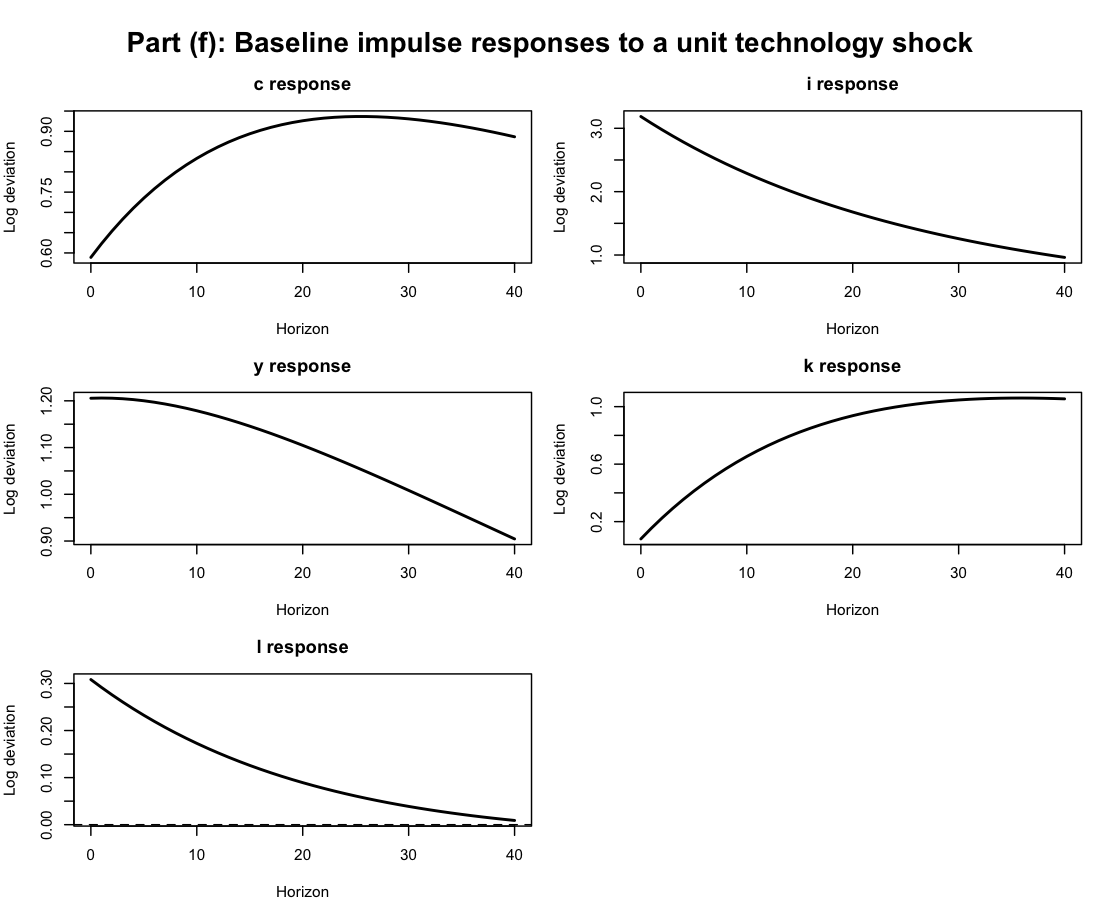
\includegraphics[width=0.8\textwidth]{hw8_part2_output/hw8_part2_baseline_irf.png}
        \caption{IRFs to a unit technology shock}
        \label{fig:hw8_f}
    \end{figure}

    Following a positive technology shock, all variables increase on impact. Consumption and capital rise gradually and converge to higher steady-state levels. Investment is initially high but declines over time as capital accumulates. Output rises on impact but decreases thereafter toward its long-run level. Labor declines monotonically due to the wealth effect and converges back to steady state.

    \newpage
    \item We show the comparison parameter by parameter.
    
    Figure \eqref{fig:hw8_g_eta} shows the comparison of $\eta$.
    \begin{figure}[H]
        \centering
        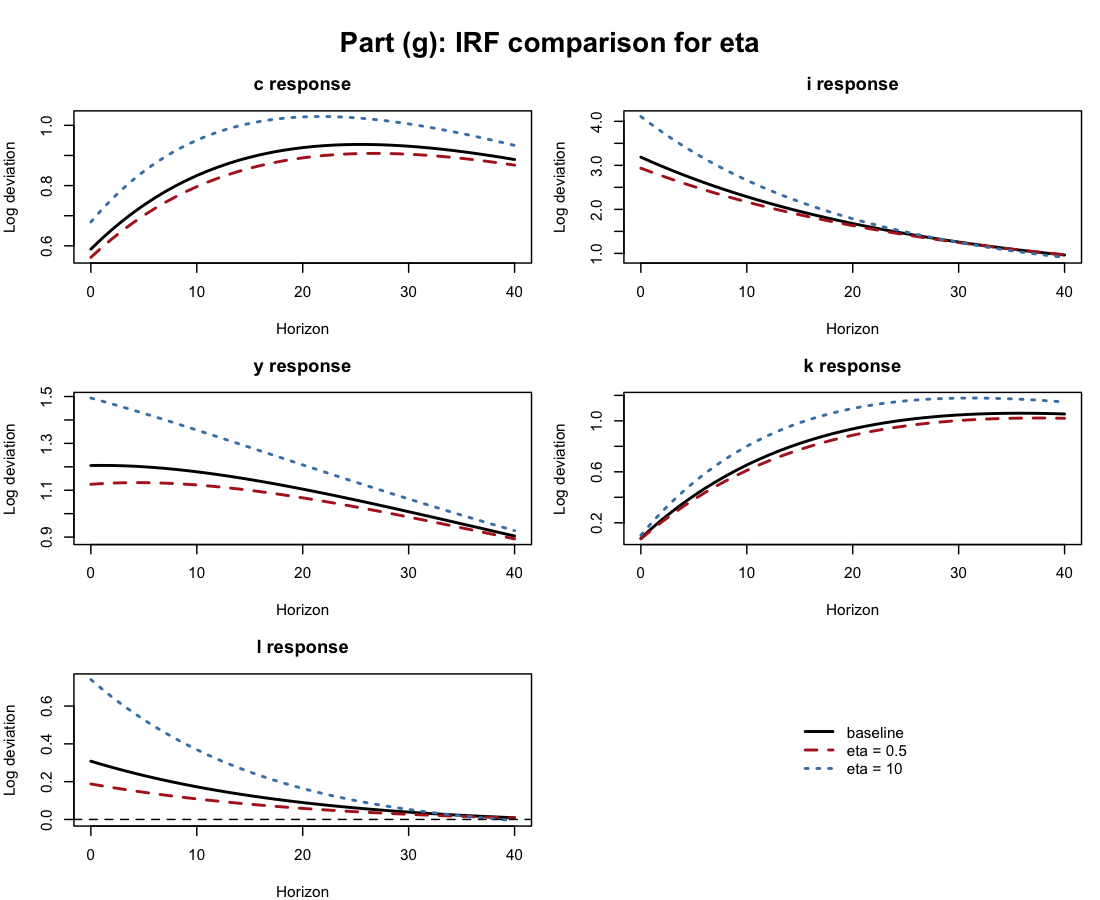
\includegraphics[width=0.8\textwidth]{hw8_part2_output/hw8_part2_eta_comparison_irf.png}
        \caption{Comparison of $\eta$}
        \label{fig:hw8_g_eta}
    \end{figure}
    
    $\eta$ is the Frisch elasticity of labour supply. A higher $\eta$ means that workers are more responsive to changes in real wages. After a positive productivity shock, real wage increases so that labour hours increase more when $\eta$ is higher. As a result, output increases more, consumption increases more, investment increases more right after the shock. As a result, capital accumulation is faster.
    
    \newpage
    Figure \eqref{fig:hw8_g_phi} shows the comparison of $\phi$.
    \begin{figure}[H]
        \centering
        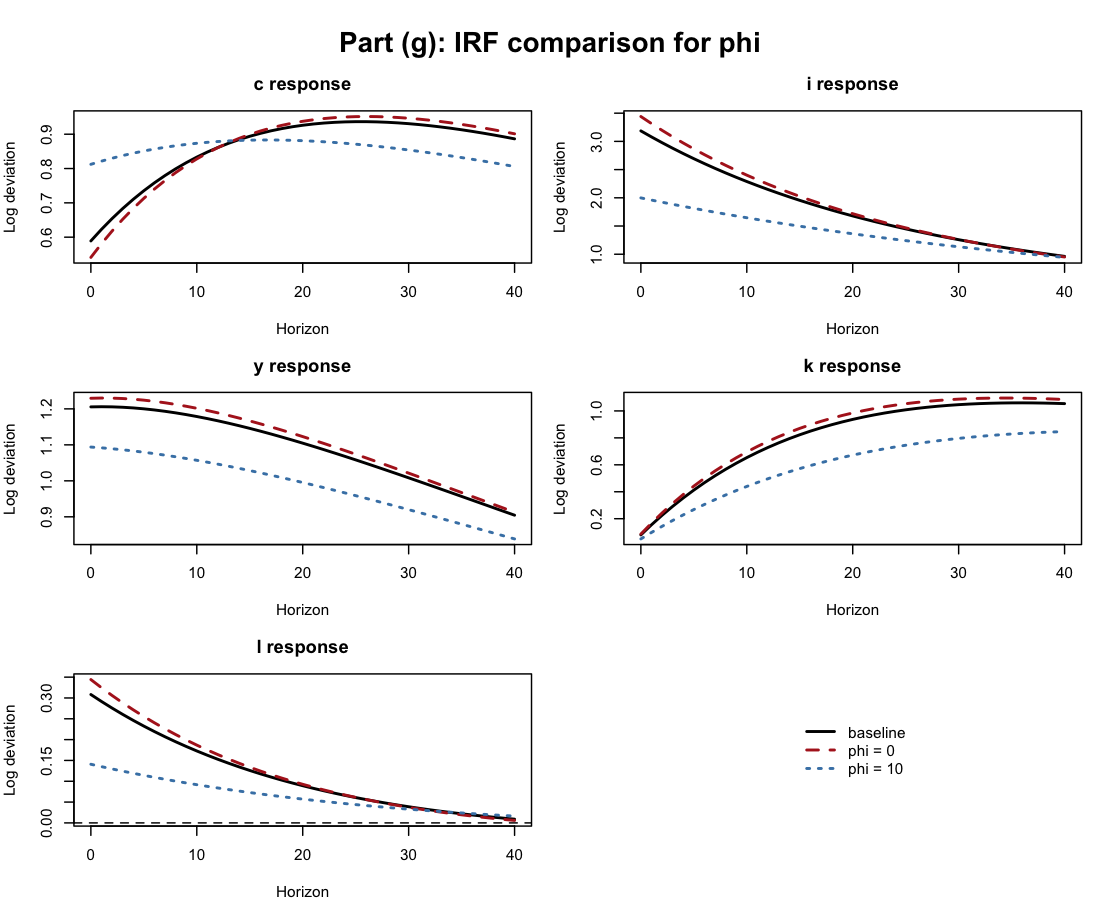
\includegraphics[width=0.8\textwidth]{hw8_part2_output/hw8_part2_phi_comparison_irf.png}
        \caption{Comparison of $\phi$}
        \label{fig:hw8_g_phi}
    \end{figure}
    
    $\phi$ is the adjustment cost parameter. A higher $\phi$ means that it is more costly to adjust capital stock. This limits the extent to which output and investment increase. Since investment cannot respond as much, consumption rises more than the baseline. Labour increases less than the baseline due to the smaller response of real wage. In the long-run, capital stock converges to a lower steady-state due to the higher adjustment cost, and so do output and consumption.

    \newpage
    Figure \eqref{fig:hw8_g_sigma} shows the comparison of $\sigma$.
    \begin{figure}[H]
        \centering
        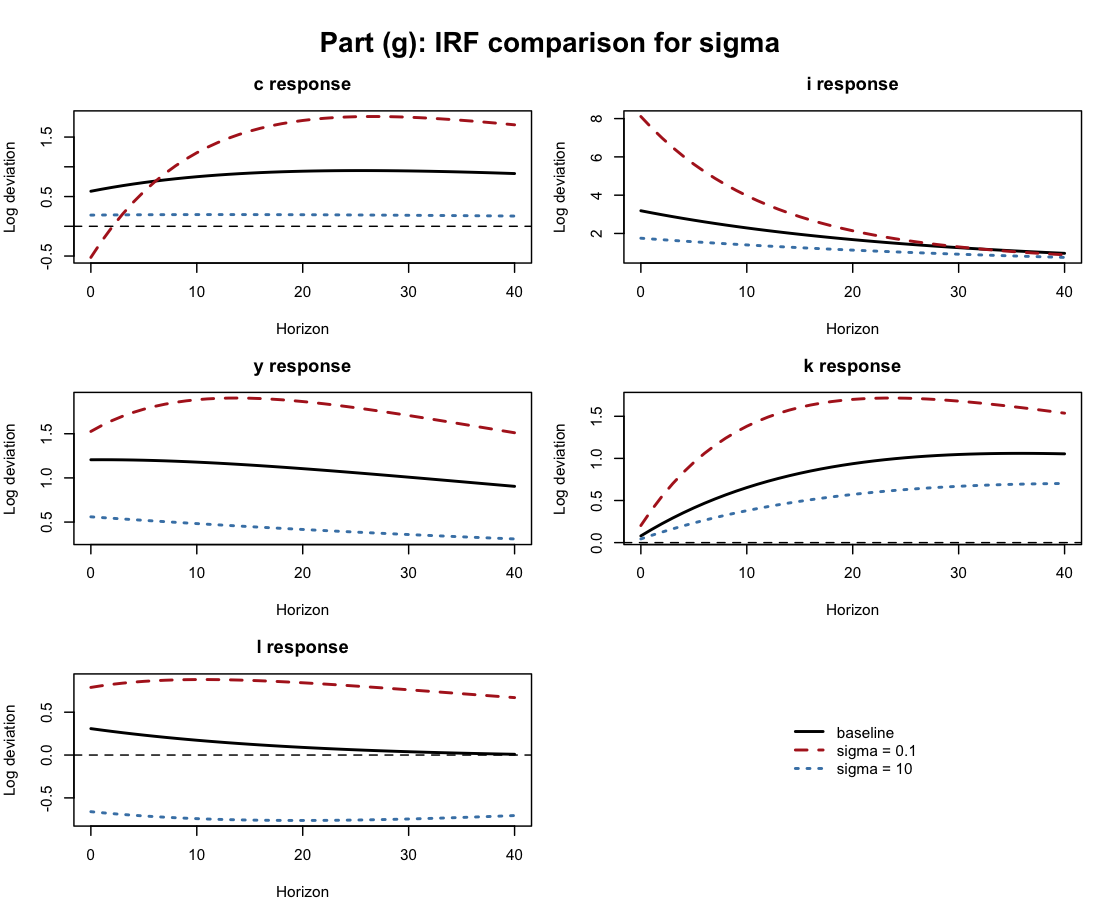
\includegraphics[width=0.8\textwidth]{hw8_part2_output/hw8_part2_sigma_comparison_irf.png}
        \caption{Comparison of $\sigma$}
        \label{fig:hw8_g_sigma}
    \end{figure}
    
    $1 / \sigma$ is the intertemporal elasticity of substitution.When $\sigma = 10$, the IES is small, meaning that consumers are reluctant to change their consumption. As a result, consumption increases less and output increases less. As the consumption smoothing effect is strong, a higher real wage leads to less labour supply, so labour drops after the shock. Investment also increases less due to the consumption smoothing incentive. When $\sigma = 0.1$, the IES is large, meaning that consumers are willing to consume in the future. As a result, consumption drops immediately after the shock but rises to a higher value in the long run. This incentive also leads to an increase in labour to gain more income, and higher saving (investment), and thus higher output and capital stock.

    \newpage
    Figure \eqref{fig:hw8_g_rho} shows the comparison of $\rho$.
    \begin{figure}[H]
        \centering
        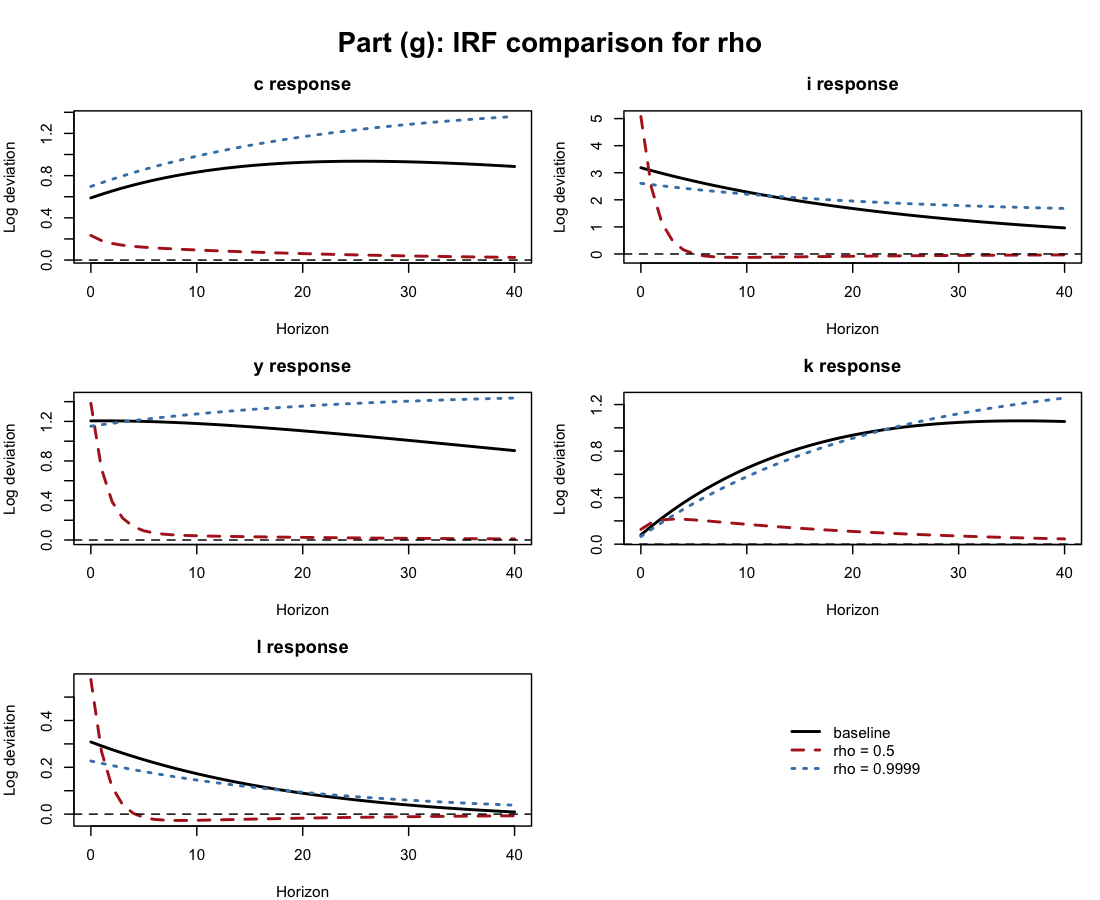
\includegraphics[width=0.8\textwidth]{hw8_part2_output/hw8_part2_rho_comparison_irf.png}
        \caption{Comparison of $\rho$}
        \label{fig:hw8_g_rho}
    \end{figure}
    
    $\rho$ is the persistence of the technology shock. A higher $\rho$ means that the technology shock is more persistent. This is straightforward to see from the IRFs.

    \newpage
    \item Table \ref{tab:hw8_h} summarizes the variance-coveriance matrix.
    \begin{table}[H]
        \centering
        \caption{Variance-Covariance Matrix of Variables}
        \label{tab:hw8_h}
        \begin{tabular}{lcccc}
        \hline
         & $dc$ & $dy$ & $d\ell$ & $di$ \\
        \hline
        $dc$ & 1.7295 & 3.4489 & 0.8597 & 8.9721 \\
        $dy$ & 3.4489 & 7.0667 & 1.8089 & 18.6871 \\
        $d\ell$ & 0.8597 & 1.8089 & 0.4746 & 4.8575 \\
        $di$ & 8.9721 & 18.6871 & 4.8575 & 49.8930 \\
        \hline
        \end{tabular}
        \\[0.5em]
        \footnotesize{Note: All entries are expressed in units of $10^{-5}$.}
    \end{table}

    For the data counterpart, I use \texttt{real gross domestic product}, \texttt{real personal consumption expenditures}, \texttt{average weekly hours of all employees}, and \texttt{gross private domestic investment} from FRED. Table \ref{tab:hw8_h_data} shows the variance-covariance matrix of the HP-filtered data counterparts. VAR is not used for this question.

    \begin{table}[H]
        \centering
        \caption{Variance-Covariance Matrix of Variables (HP-Filtered Data Analogues)}
        \label{tab:hw8_h_data}
        \begin{tabular}{lcccc}
        \hline
         & $dC$ & $dY$ & $dL$ & $dI$ \\
        \hline
        $dC$ & 24.3422 & 19.7796 & 1.6201 & 57.2742 \\
        $dY$ & 19.7796 & 18.9462 & 1.8634 & 65.7208 \\
        $dL$ & 1.6201 & 1.8634 & 1.7509 & 14.9673 \\
        $dI$ & 57.2742 & 65.7208 & 14.9673 & 382.6942 \\
        \hline
        \end{tabular}
        \\[0.5em]
        \footnotesize{Note: All entries are expressed in units of $10^{-5}$ using HP-filtered log data with quarterly smoothing parameter $\lambda = 1600$.}
    \end{table}

    The magnitudes differ a lot. The main reason may be that the model only considers the TFP shock while the data counterparts experiece much more shocks than the TFP shock. There is also the magnitude issue, where the aggregate data seems much larger than the normalized model.

    \item Main variables respond in a similar pattern except labour. My results show that labour hour increases while Gali's VAR result shows that labour hour decreases. The main difference is that Gali's model incorporates money. In a monetary model, when labour is introduces, money neutrality does not hold and money growth affect labour supply decision. In this model, the mechanism is such that a positive productivity growth increases the real wage which leads to higher labour supply. In Gali's model, when the coefficient of lagged TFP shock is positive in the money growth process, a positive productivity growth leads to higher expected inflation and thus a higher nominal interest rate. As a result, people hold less money and thus less consumption. As a result, labour hours decrease.

    \newpage
    \noindent\textbf{Part III}
    \item With government spending, at steady state, \eqref{eq:ss_consumption_investment} becomes
    \begin{align}\label{eq:ss_consumption_investment_gov}
        Y^* = C^* + I^* + G^*.
    \end{align}
    where $G^*$ is the government spending. There is an additional relation at steady state:
    \begin{align}\label{eq:ss_gov_relation}
        G^* = 0.2 Y^*.
    \end{align}
    With one more variable and one more equation, the system is still solvable.

    In the log-linearized system, \eqref{eq:ll_consumption_investment} becomes
    \begin{align}\label{eq:ll_consumption_investment_gov}
        \hat{y}_t = \hat{c}_t \frac{C^*}{Y^*} + \hat{\iota}_t \frac{I^*}{Y^*} + 0.2 \hat{g}_t.
    \end{align}
    where $\hat{g}_t$ is the log-linearized government spending. The grovernment spending process provides one more equation:
    \begin{align}\label{eq:ll_gov_process}
        \hat{g}_t = \psi \hat{g}_{t-1} + u_t.
    \end{align}

    The impulse response comparisons are in Figure \ref{fig:hw8_i}.
    \begin{figure}[H]
        \centering
        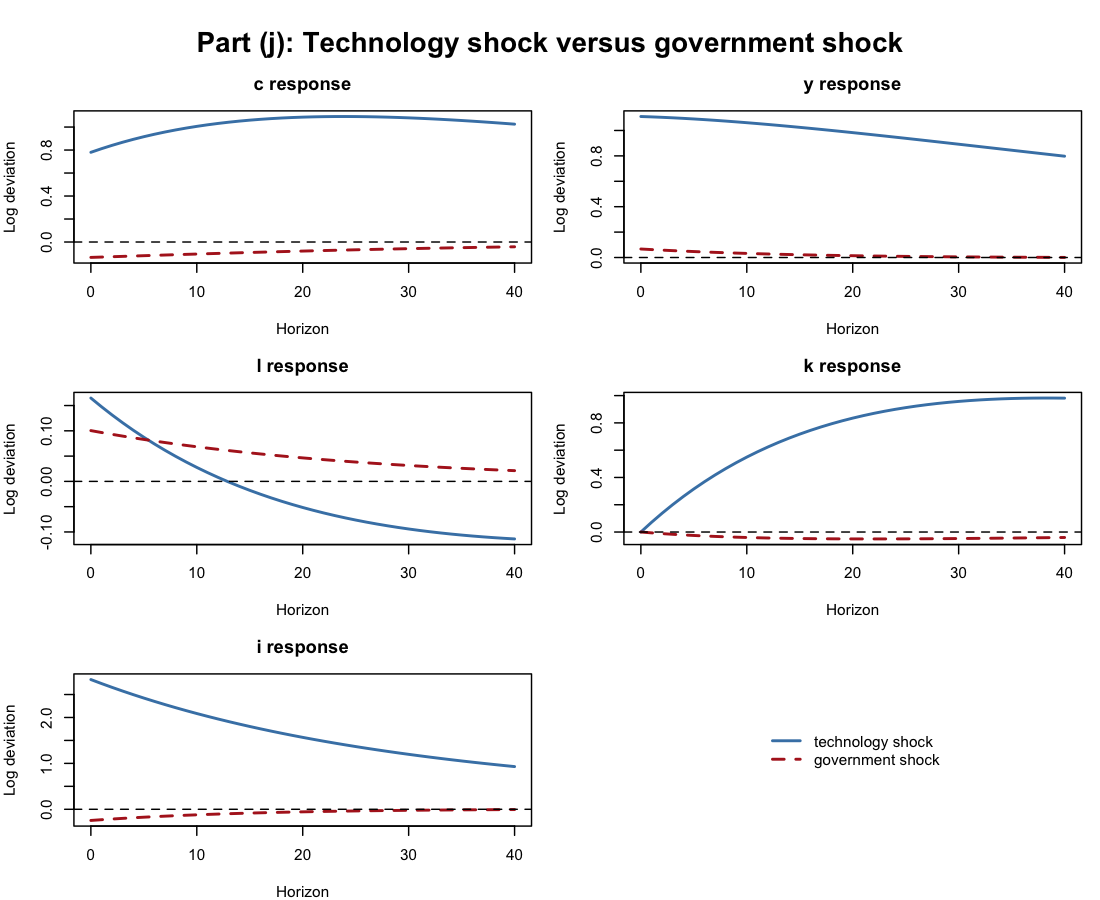
\includegraphics[width=0.8\textwidth]{hw8_part3_output/hw8_part3_j_irf_comparison.png}
        \caption{Impulse response comparisons}
        \label{fig:hw8_i}
        \footnotesize{Note: This TFP shock is in the system with government spending.}
    \end{figure}

    An increase in government spending increases output. However, it occupies part of consumption and investment so consumption and investment decrease. Capital stock decreases as a result. As consumption decreases, MUC increases and thus labour supply increases to obtain more resources.

    \newpage
    \item Figure \ref{fig:hw8_j} shows the FEVDs.
    \begin{figure}[H]
        \centering
        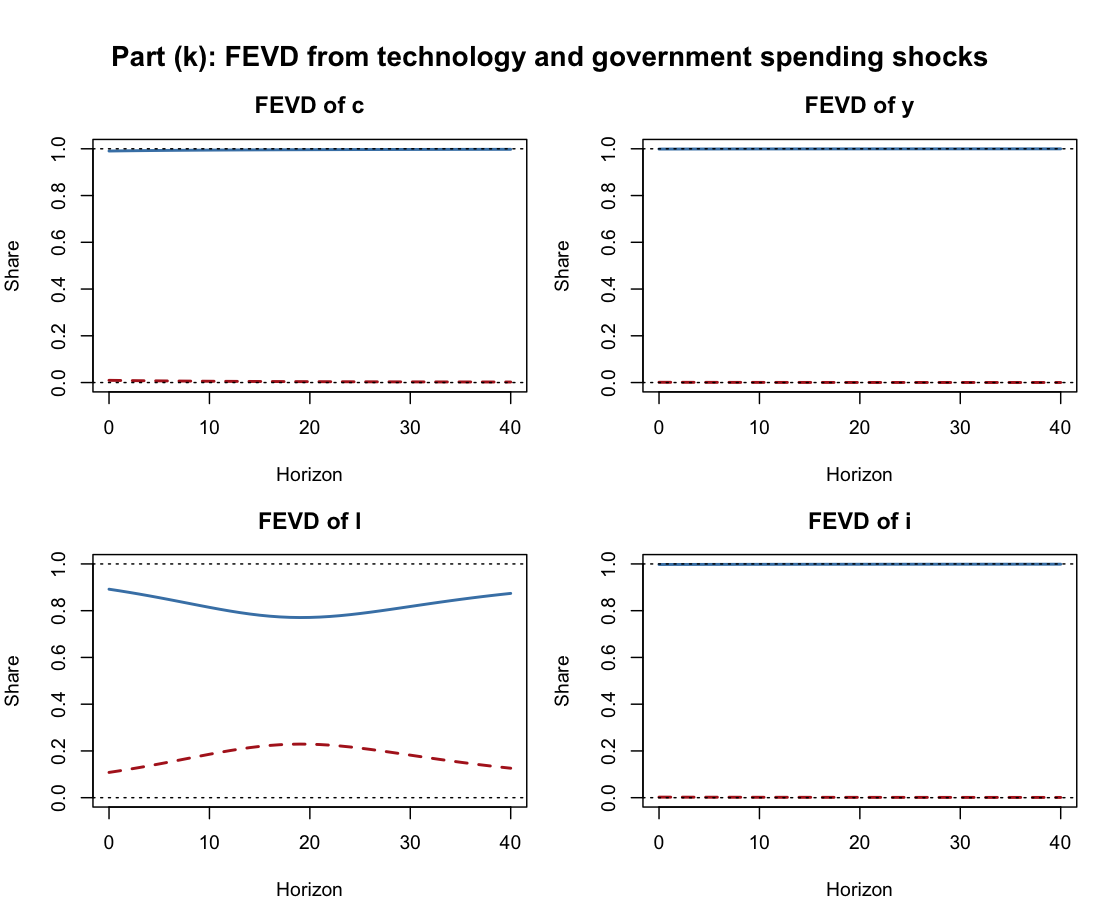
\includegraphics[width=0.8\textwidth]{hw8_part3_output/hw8_part3_k_fevd.png}
        \caption{FEVDs}
        \label{fig:hw8_j}
    \end{figure}

    The TFP shock almost account for all the variances of consumption, output and investment. This is because government spending only enters the system through the resource constraint while the TFP shock directly enters the production function. Labour supply is affected relatively more by the government spending shock than the other three variables. This is because even without a TFP shock, the above-mentioned MUC will works much to drive this change.
\end{enumerate}

\end{document}